
It originates in \textcite{scvo85} (1985). 

\begin{center}
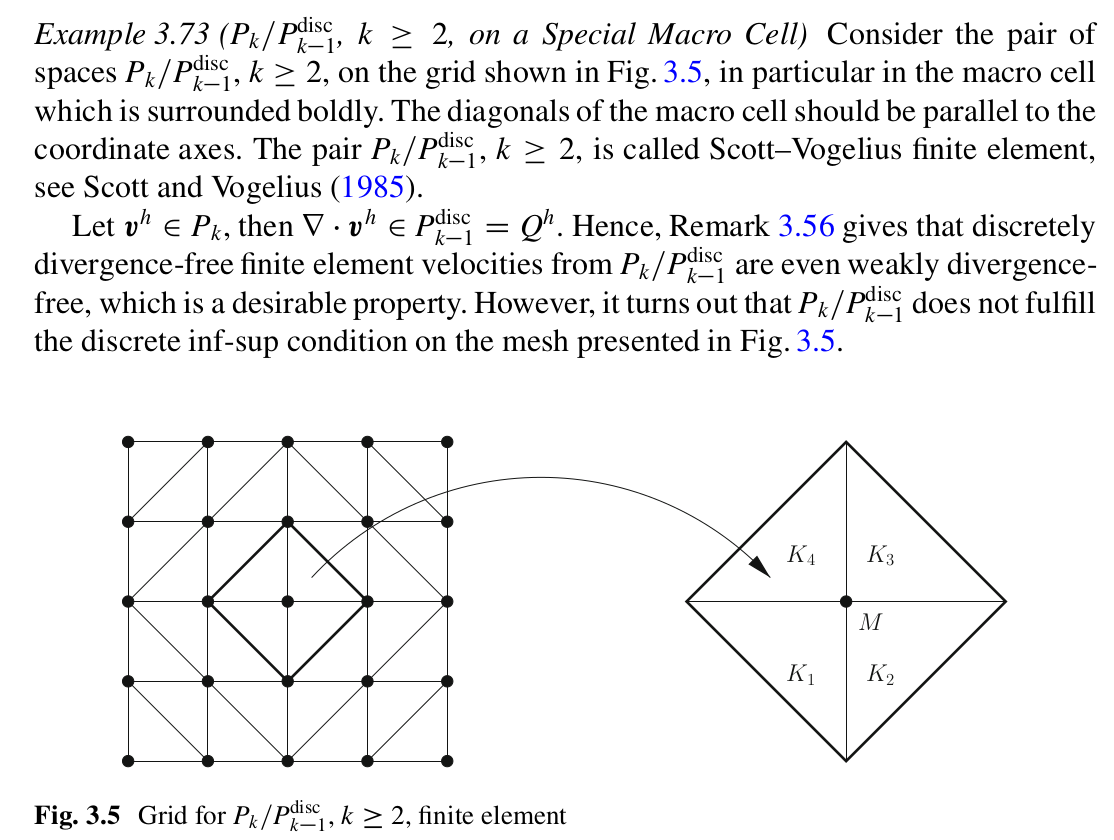
\includegraphics[width=10cm]{images/pair_scott_vogelius/john_scott_vogelius}\\
\captionfont{Taken from John \cite[p70]{john16}.} 
\end{center}

See also \textcite{jolm17} (2017). 

Chen [ref?!] says: ($P^k ,P^{k-1}$) : stable if $k \ge 4$ in $R^2$ and for meshes without
singular-vertex. Exact divergence free. Not easy to code due to the high degree.


